\chapter[Experiment]{Experiment Evaluation}
\label{exp}

	\section{Introduction}
	\label{exp:intro}

		As a way to get the widest possible range of data from the scenes created, two different experiments were planned (\enquote{Experiment 1}, and \enquote{Experiment 2}).
		The experiments were set up in a way that a participant in an experiment would either be shown the standard or non-Euclidean game scene first, and once they had successfully navigated around it, they would then be shown the other.
		\enquote{Experiment 1} had the participants viewing the standard scene first and the non-Euclidean scene second, with \enquote{Experiment 2} having the participants view the non-Euclidean scene first and the standard scene second.

		A total of 10 participants took part in the experiments, with 5 participants taking part in \enquote{Experiment 1}, and the other 5 \enquote{Experiment 2}.
		Having the participants view the two scenes in different orders allowed for the results of the experiments to not only cover the effects of the respective scenes geometry, but also to see if being exposed to the other environment in any way impacts their immersion to the one they are currently in. % TODO: Reword this

		During the experiments, participants were asked to fill out a 2 page questionnaire, a blank version of which can be seen on page \pageref{appendix:question}.
		After viewing the first scene, participants were asked to fill out the first page of the questionnaire. Once they'd filled the page, they would view the second scene, after which they were asked to fill out the second page. % TODO: Reword this
		All participants were naive to the purpose of the experiments.

		An Oculus Rift Developer Kit 2 was used as the display device for the experiments, using the supplied IR camera for six degrees of freedom head tracking within the scenes.
		The same desktop computer was used for all experiments (CPU: Intel Core i7 4790, GPU: NVIDIA GTX 970, RAM: 16GB), to ensure consistent render speeds for each participant.

		The analysis of the gathered results will be covered in three sections. The first will cover the results from all 10 experiments solely on the data gathered for the standard scene; The second covers the results from all 10 experiments solely on the data from the non-Euclidean scene; Finally, the third covers the comparison between the two scene types depending on the order of viewing. % TODO: Reword this?

		% REMEMBER TO SPEAK ABOUT THE MATHS

	\section{Experiments}
	\label{exp:exp}

		\subsection{Standard Euclidean Geometry}
		\label{exp:exp:standard}

			Having an experiment scene using standard Euclidean geometry which follows a similar layout to the non-Euclidean scene sets a good foundation for the validation of the results. % TODO: Reword this?
			The questionnaire the participants were asked to fill in focused on two main metrics, their personal sense of immersion within the scene, as well as their sense of comfort navigating within the scene.

			% Talk about the results specific to the standard euclidean geometery here.
			% Used to get a base result for immersion
			% Consistent high ratings for immersion
			% Navigation comfort was varied, but talk about the high mean values

			% IMMERSION MEAN:  7
			% IMMERSION STDEV: 1 - LOWER SD MEANS LESS VARIANCE
			% COMFORT MEAN:    7
			% COMFORT STDEV:   2

			\begin{figure}[H]
				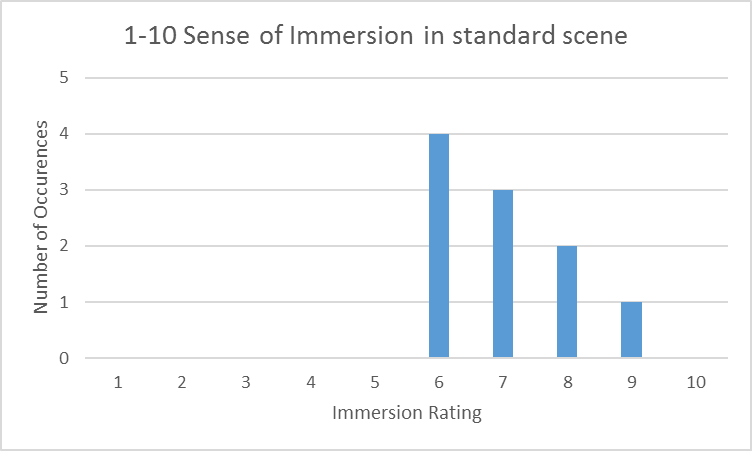
\includegraphics[width=0.7\textwidth]{Images/Standard_Immersion}
				\centering
				\caption{Immersion rating in standard geometry test scene}
				\label{exp:fig:standard_immersion}
			\end{figure}

			\begin{figure}[H]
				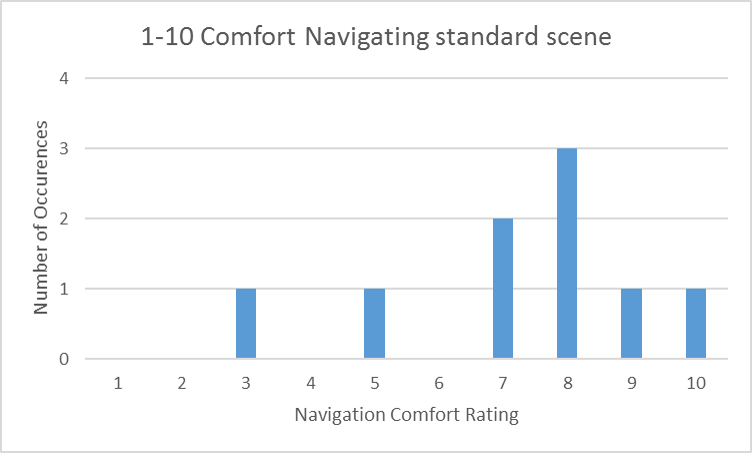
\includegraphics[width=0.7\textwidth]{Images/Standard_Comfort}
				\centering
				\caption{Navigation Comfort rating in standard geometry test scene}
				\label{exp:fig:standard_comfort}
			\end{figure}

			\begin{figure}[H]
				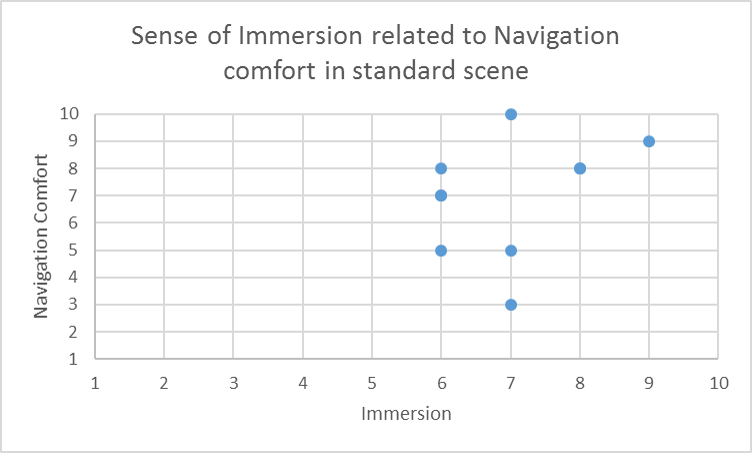
\includegraphics[width=0.7\textwidth]{Images/Standard_Relation}
				\centering
				\caption{Relation between sense of immersion and navigation comfort in standard geometry test scene}
				\label{exp:fig:standard_relation}
			\end{figure}

		\subsection{Non-Euclidean Geometry}
		\label{exp:exp:ne}

			Similarly to the standard Euclidean scene, after viewing the non-Euclidean scene participants were asked to answer questions relating to two main metrics, their sense of immersion, and comfort navigating the scene.

			% Talk about the results specific to the non-eucldean geometry here
			% More varied results
			% Same Mean
			% More responses in the higher end of the scale - talk about the written feedback
			% Lower comfort with navigation

			% IMMERSION MEAN:  7
			% IMMERSION STDEV: 1.342 (4SF)
			% COMFORT MEAN:    6.2
			% COMFORT STDEV:   1.6

			\begin{figure}[H]
				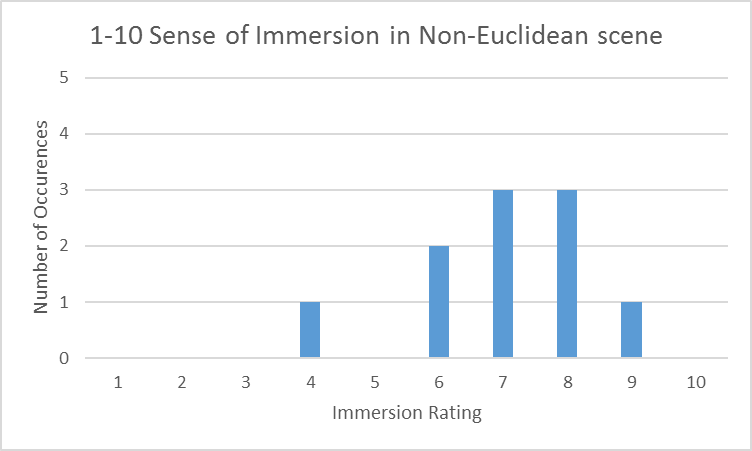
\includegraphics[width=0.7\textwidth]{Images/NE_Immersion}
				\centering
				\caption{Immersion rating in Non-Euclidean geometry test scene}
				\label{exp:fig:ne_immersion}
			\end{figure}

			\begin{figure}[H]
				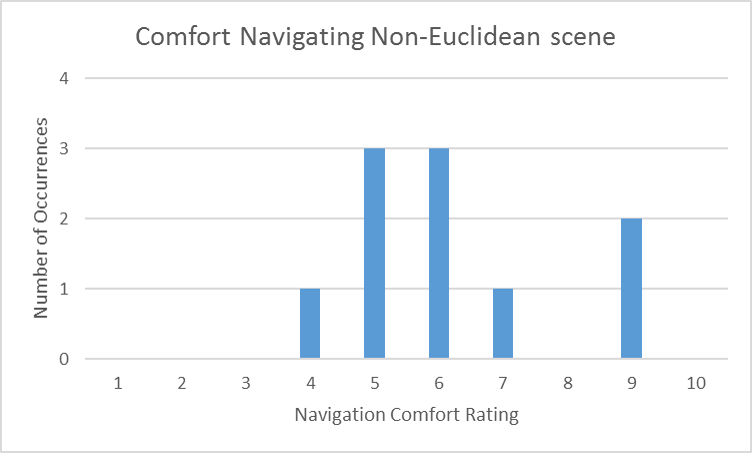
\includegraphics[width=0.7\textwidth]{Images/NE_Comfort}
				\centering
				\caption{Navigation Comfort rating in Non-Euclidean geometry test scene}
				\label{exp:fig:ne_comfort}
			\end{figure}

			\begin{figure}[H]
				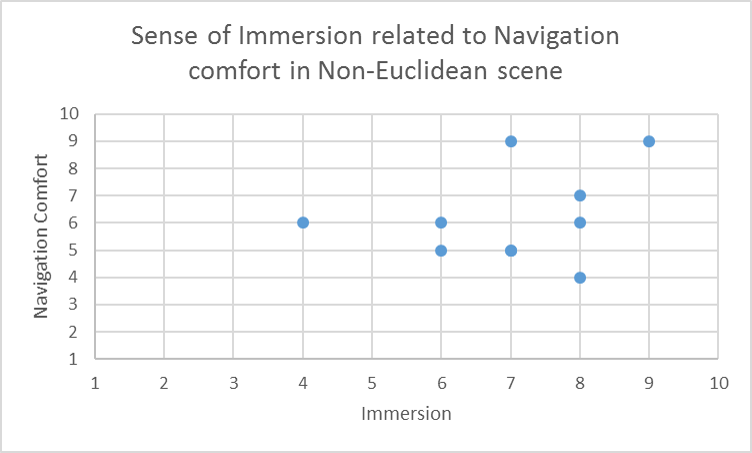
\includegraphics[width=0.7\textwidth]{Images/NE_Relation}
				\centering
				\caption{Relation between sense of immersion and navigation comfort in Non-Euclidean geometry test scene}
				\label{exp:fig:ne_relation}
			\end{figure}

		\subsection{Comparisons}
		\label{exp:exp:comp}

			With the results of both individual scenes gathered and analysed, 

			% 5 Participants took part in exp 1, 5 in exp 2.
			% exp 1 40% of participants had not used a VR system previously.
			% exp 2 20% of participants had not used a VR system previously.

			% Experiment 1 was Standard First
			% Experiment 2 was NE First
			% Talk about the comparisons
			% Talk about how the data MEANs something
			% Participants from exp1 never felt that NE was less immersive, either as immersive or more - quote feedback - \enquote{The puzzling nature of exploring a familiar map that is no longer familiar} was a positive impact on immersion
			% Participants from exp2 varied a lot more, sometimes NE was more immersive, sometimes  the same, sometimes less so.

			\begin{figure}[H]
				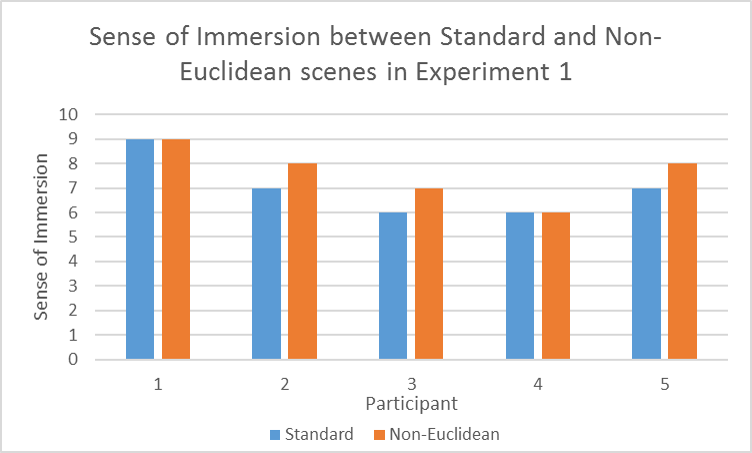
\includegraphics[width=0.7\textwidth]{Images/Compare_Immersion_Exp_1}
				\centering
				\caption{Comparison of participants sense of immersion in the two test scenes, from Experiment 1}
				\label{exp:fig:compare_immersion_exp1}
			\end{figure}

			\begin{figure}[H]
				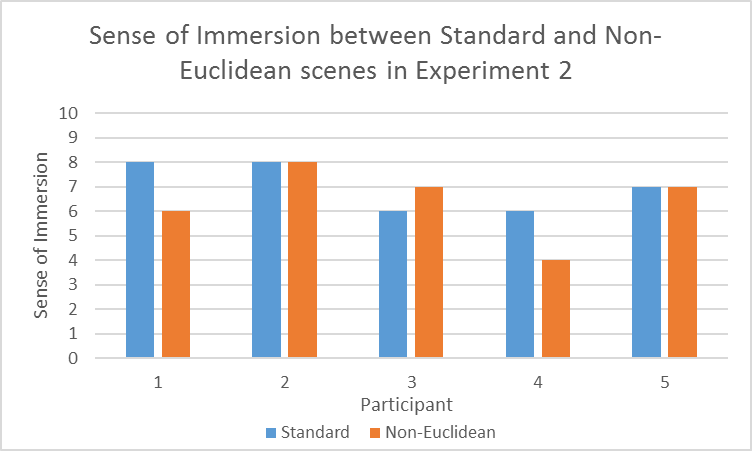
\includegraphics[width=0.7\textwidth]{Images/Compare_Immersion_Exp_2}
				\centering
				\caption{Comparison of participants sense of immersion in the two test scenes, from Experiment 2}
				\label{exp:fig:compare_immersion_exp2}
			\end{figure}

			\begin{figure}[H]
				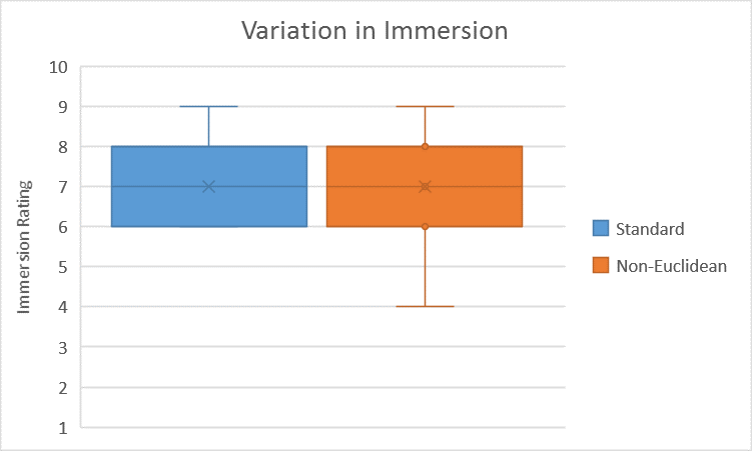
\includegraphics[width=0.7\textwidth]{Images/Compare_Immersion_Variation}
				\centering
				\caption{Mean values, and variation of Range for Immersion in the two test scenes}
				\label{exp:fig:compare_immersion_variation}
			\end{figure}

	\section{Summary}
	\label{exp:summary}

		The results of the experiments as a whole are interesting in the sense that they go against original expectations.

		% TODO - Here I will be evaluating the results of the experiments, covering any trends that appeared between the various experiments, discussing potential impacts from the results, as well as covering any additional notes that were provided about the experiments from the participants which weren't directly related to the specific experiment they were part of.

		% Results show that an NE environment can be more immersive than a standard env, so long as the user has had a chance to familiarise themselves in a standard euclid setting first
		% More work needs doing to improve upon the navigation side, there were mixed reviews from both scenes and experiments - quote feedback - room for further study
